% Slides for 2024-04-29
% To create a slide, use the following:
% \begin{frame}{TITLE}
%     BODY
% \end{frame}

% To create a slide with a bullet list, use the following:
% \begin{frame}{TITLE}
%     \begin{itemize}
%         \item ITEM 1
%         \item ITEM 2
%     \end{itemize}    
% \end{frame}

% To create a slide with numbered list, use the following:
% \begin{frame}{TITLE}
%     \begin{enumerate}
%         \item ITEM 1
%         \item ITEM 2
%     \end{enumerate}
% \end{frame}

% To create a slide with a graphic:
% 1. Add the graphic to this folder (named picture.png)
% 2. Use the following:
% \begin{frame}{TITLE}
%     \centering
%     \includegraphics[height=0.7\textheight,width=0.7\textwidth,keepaspectratio]{picture.png}
% \end{frame}

% To create a slide with two columns, use the following:
% \begin{frame}{TITLE}
%     \begin{columns}
%         \begin{column}{0.5\textwidth}
%             COLUMN 1 BODY
%         \end{column}
%         \begin{column}{0.5\textwidth}
%             COLUMN 2 BODY
%         \end{column}
%     \end{columns}
% \end{frame}

\begin{frame}{Frontend Candidate Interviews}
    Ready to send acceptance/rejection notices
\end{frame}

\begin{frame}{User Request Refactoring}
    Preprocessing now accepts:
    \begin{enumerate}
        \item Multiple tiffs
        \item CRS
    \end{enumerate}
\end{frame}

\begin{frame}{Satellite RGB Imagery}
    \centering
    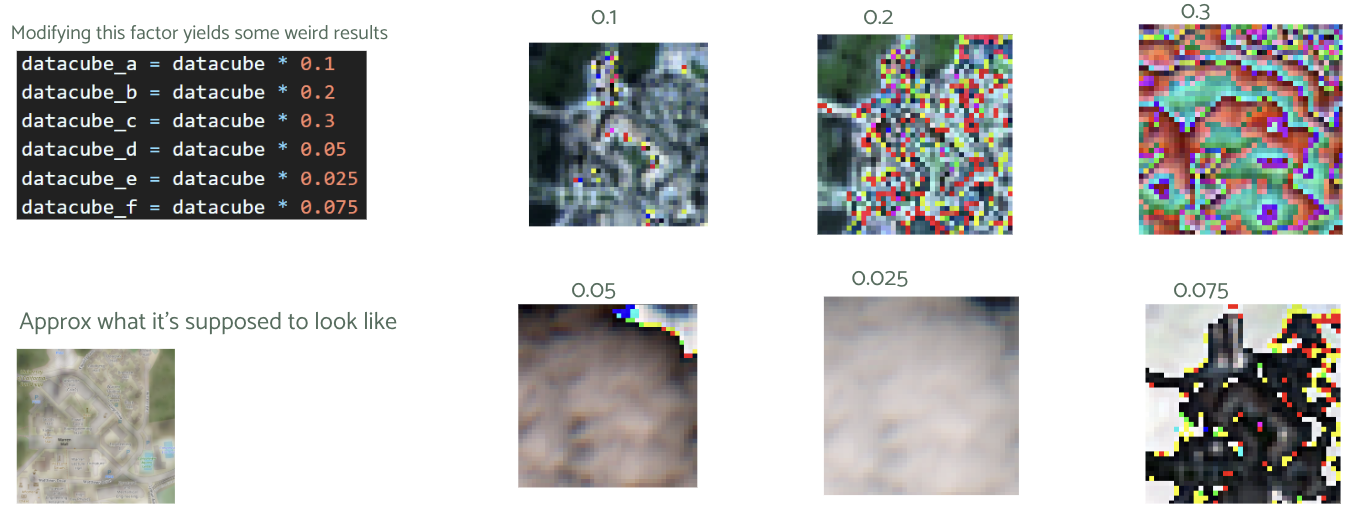
\includegraphics[height=0.7\textheight,width=0.7\textwidth,keepaspectratio]{images/mm-rgbsat.png}
\end{frame}

\begin{frame}{Model Learning Kind of?}
    \centering
    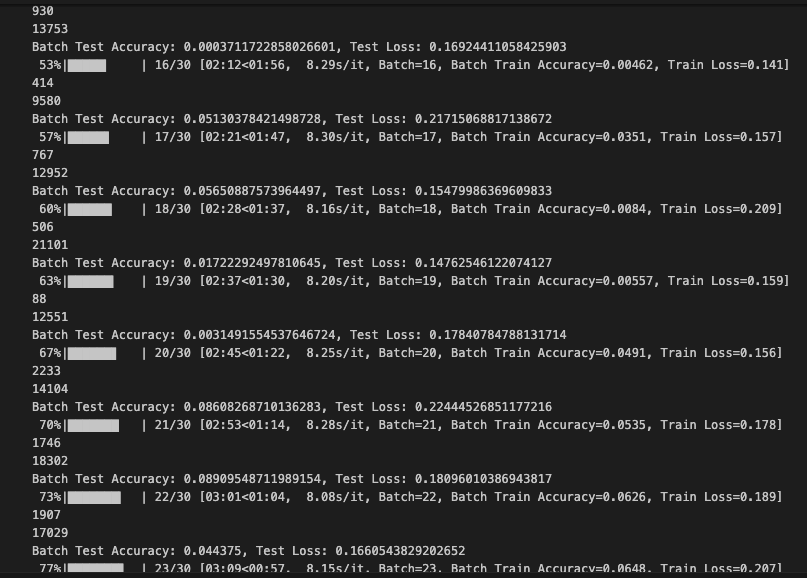
\includegraphics[height=0.7\textheight,width=0.7\textwidth,keepaspectratio]{images/train.png}
\end{frame}

\begin{frame}{Accuracy Graph}
    \centering
    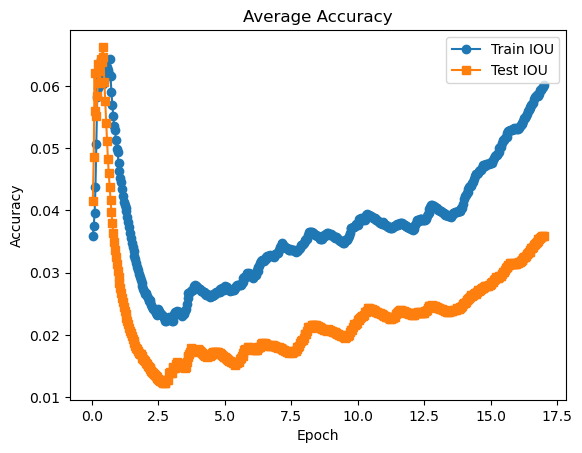
\includegraphics[height=0.7\textheight,width=0.7\textwidth,keepaspectratio]{images/Average Accuracy.png}
\end{frame}

\begin{frame}{Hugh's Updates}
    \url{https://drive.google.com/file/d/1gVdLHgWHzqVSYEmdD014OFJR5qnPpjux/view?usp=drive_link}
\end{frame}
